%//////////////////////////////////////////////////////////////////////////////////////////////////////////////////////////////////////////////////////

\section{The Large Hadron Collider}
\label{sec:LHC}

%//////////////////////////////////////////////////////////////////////////////////////////////////////////////////////////////////////////////////////

The Large Hadron Collider (LHC)~\cite{1748-0221-3-08-S08001} is a proton-proton (pp) collider located at the European Particle Physics Laboratory (CERN) near Geneva, Switzerland. It is situated in the former CERN Large Electron-Positron Collider (LEP) tunnel with a circumference of 27\unit{km} about 100\unit{m} under ground crossing the border between France and Switzerland. A hadron collider has been chosen to allow higher center-of-mass energies ($\sqrt{s}$) compared to electron-positron colliders, the latter limited by synchrotron radiation due to the low mass of the particles to be accelerated. High center-of-mass energies are required for the production of heavy SM particles such as the top quark and the Higgs boson, and to search for new BSM interactions at the TeV scale.
%heavy BSM resonances such as \cPZpr, \cPWpr or gravitons.
For this purpose, the LHC is designed to produce pp collisions up to a $\sqrt{s} = 14\TeV$, superseding previous high energy hadron colliders, such as Tevatron, by a factor of 7.
Higher center-of-mass energies lead to larger cross sections for the production of the physics processes of interest in parton-parton interactions (Fig.~\ref{fig:partonLumiRatio}), maximizing the sensitivity to new discoveries.
In addition to colliding protons, the LHC is also capable of accelerating and colliding heavy nuclei, which is, however, not considered in this work.

\begin{figure}[!htb]
 \begin{center}
  %\subfigure[]{\label{fig:partonLumiRatio_a}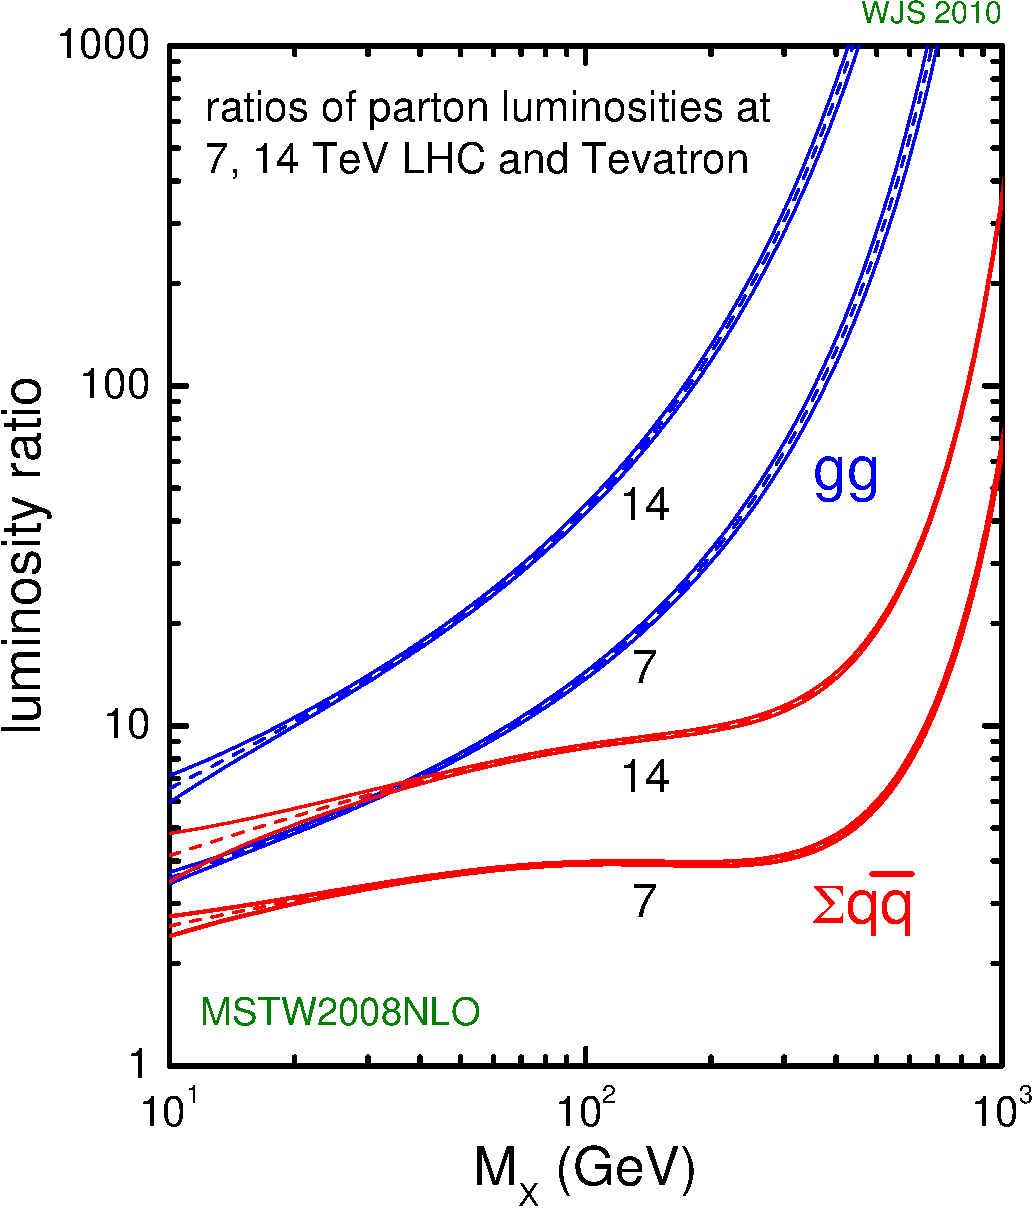
\includegraphics[width=0.25\textwidth]{\chthree/lumiTevLHC714.pdf}}
  %\subfigure[]{\label{fig:partonLumiRatio_b}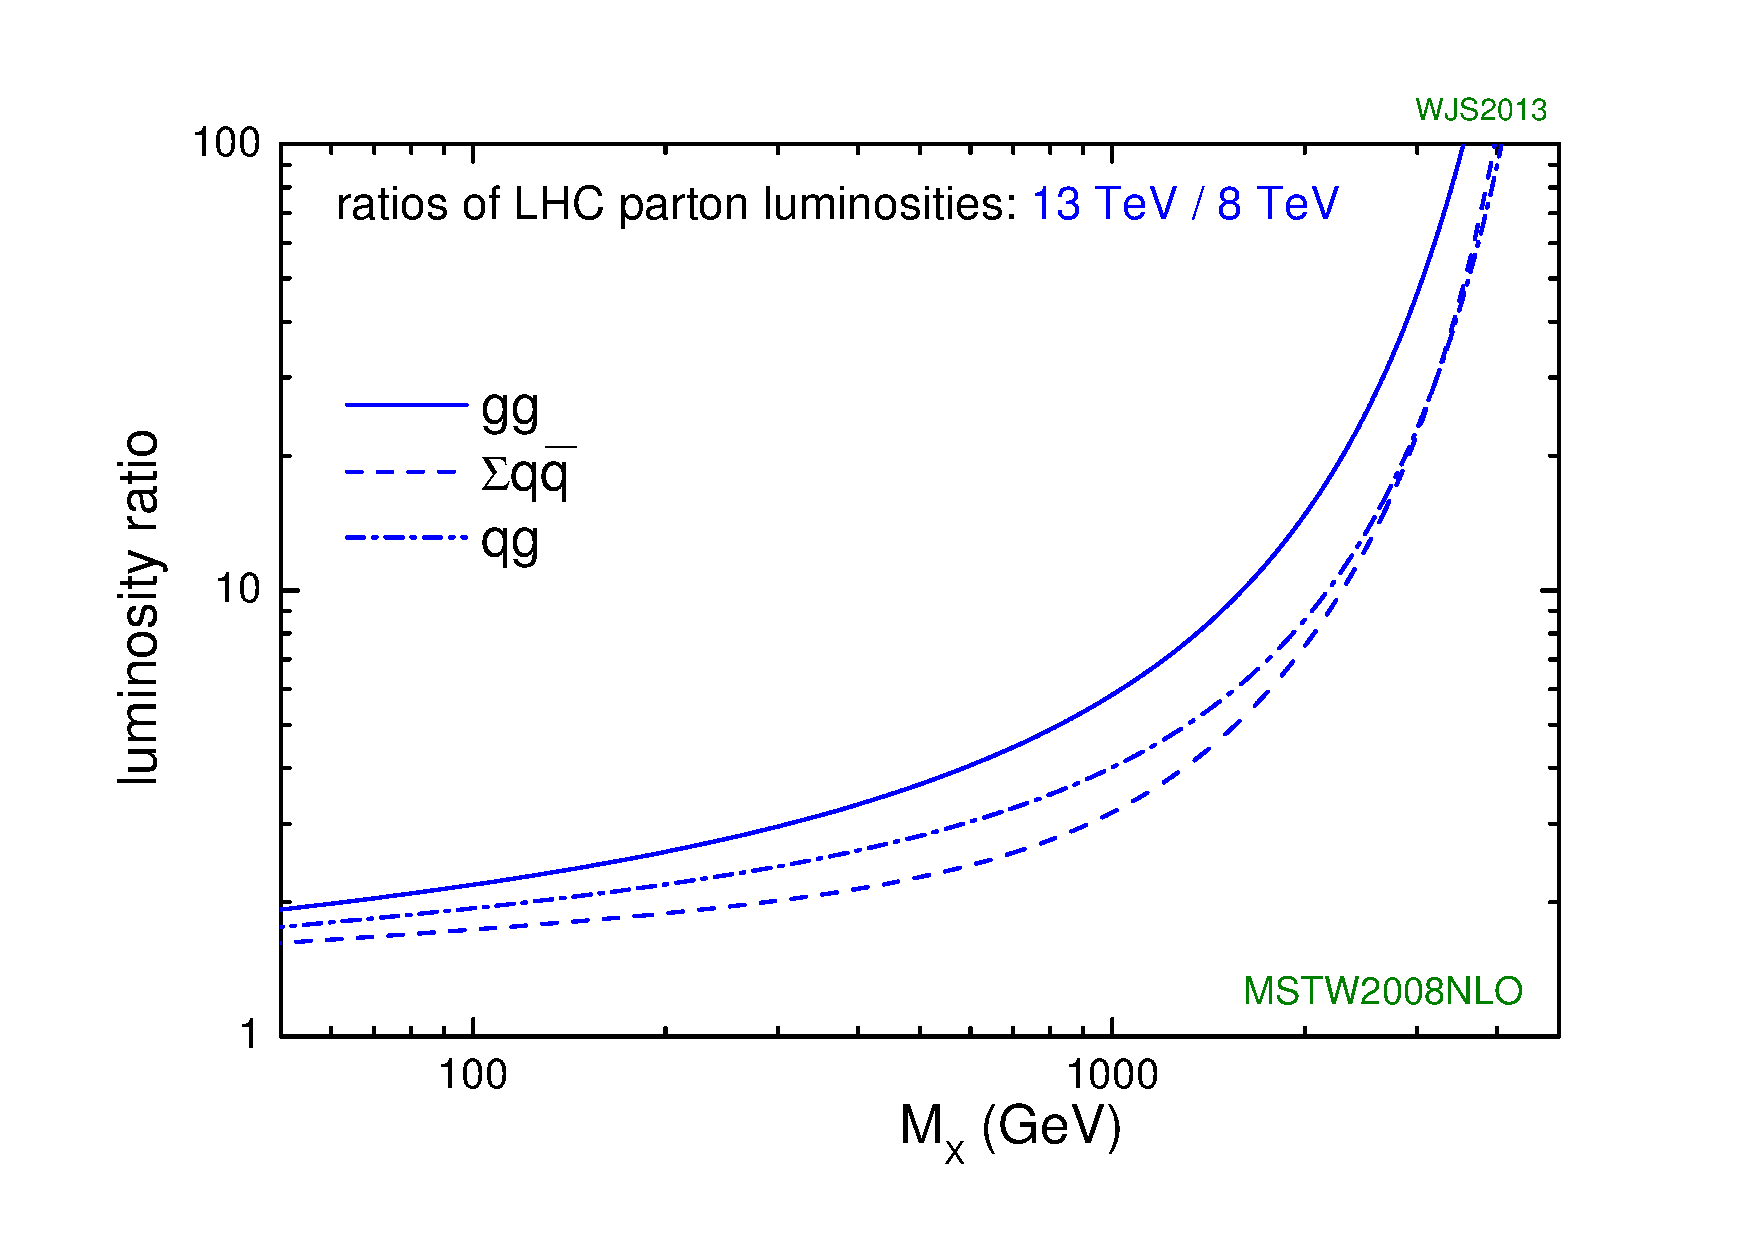
\includegraphics[width=0.46\textwidth]{\chthree/lhclumi7813_2013_v1.pdf}}
  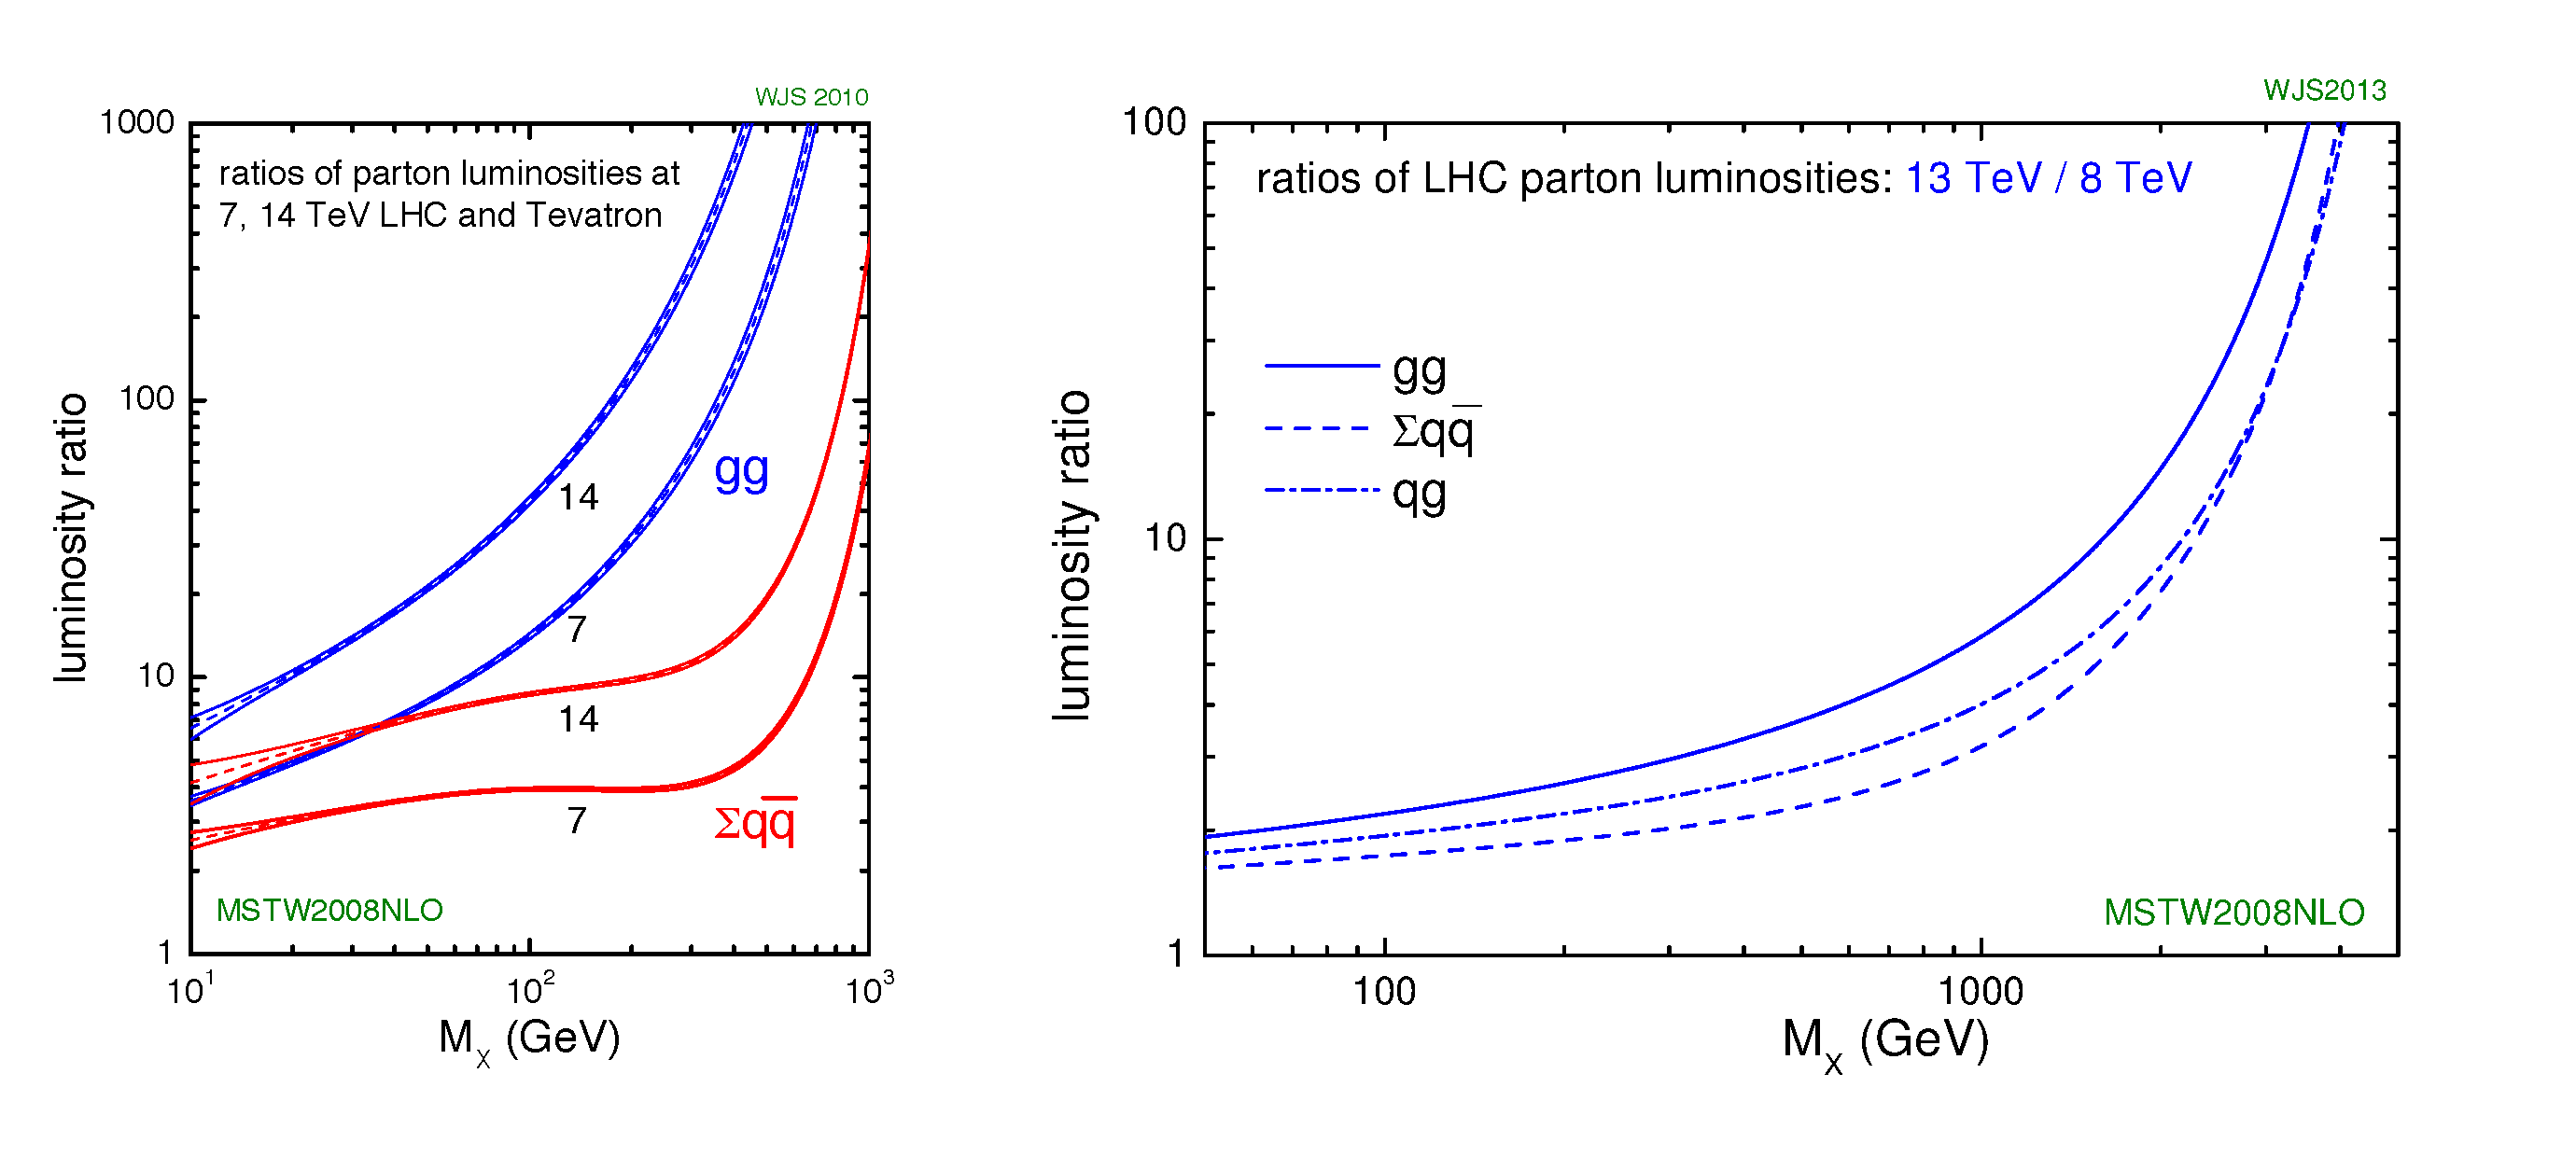
\includegraphics[width=\textwidth]{\chthree/lumiratios.pdf}
 \end{center}
 \caption{(left) Parton luminosity ratios of pp collisions at LHC at $\sqrt{s} = 7, 14\TeV$ and p$\bar{\mathrm{p}}$ collisions at Tevatron at $\sqrt{s} = 1.96\TeV$. (right) Parton luminosity ratios of pp collisions at LHC at $\sqrt{s} = 13\TeV$ and at $\sqrt{s} = 8\TeV$~\cite{LumiRatios}.}
 \label{fig:partonLumiRatio}
\end{figure}

The LHC is the final element in a succession of machines that accelerate protons to increasingly higher energies. 
%Each machine boosts the energy of a beam of protons, before injecting the beam into the next machine in the sequence. 
Protons, obtained from a hydrogen source, are first accelerated by a linear accelerator (LINAC 2) to energies of 50\MeV.
The beam is then injected into the Proton Synchrotron Booster (PSB), which accelerates the protons to 1.4\GeV, followed by the Proton Synchrotron (PS), which pushes the beam to 25\GeV. Protons are then sent to the Super Proton Synchrotron (SPS) where they are accelerated to 450\GeV.
%Using two transfer lines the protons are then injected into the two beam pipes of the LHC ring, where they circulate in opposite directions and accelerated up to the targeted energy. The LHC ring and the acceleration chain are sketched in Fig.~\ref{fig:LHC}.
Finally, the beam is injected in the LHC ring, where it completes several revolutions to reach the targeted energy. The LHC ring and the acceleration chain are sketched in Fig.~\ref{fig:LHC}.

Inside the ring, the two proton beams circulate in opposite directions in two tubes kept at ultrahigh vacuum, referred as beam pipes. The acceleration of protons inside LHC is made by radio-frequency cavities (400\unit{MHz}), giving a 492\keV energy gain per revolution, with a 7\keV loss per turn due to synchrotron radiation. It takes 4 minutes and 20 seconds to fill each LHC ring, and 20 minutes for the protons to reach their maximum energy of 7\TeV. The maximum energy of the protons is limited by the strength of the magnetic field required for keeping the protons inside the ring. For 7\TeV-protons a magnetic field of 8.3\unit{T} has to be produced, which can only be reasonably obtained by superconducting magnets. The ring is equipped with 1232 dipole magnets for bending and 392 quadrupole magnets for focussing made of niobium-titanium (NbTi), which are cooled down to a temperature of 1.9\unit{K} with the help of super-fluid helium.
%Superconducting magnets of different varieties and sizes are used to direct the beams around the accelerator.
%Among these, dipole magnets are used to bend the particle beam and to keep it into the circular tunnel. 
%There are 1232 main dipoles each 15 metres long and weighing in at 35 tonnes, which operate in a bath of liquid helium at a temperature of 1.9 K, that can provide a maximum magnetic field of 8.4 T (11850 A current).
%Additional 392 quadrupole magnets, each 5–7 metres long, are used to keep the beams focused, in order to maximize the chances of interaction between the particles in the four intersection points, where the two beams cross and the particle detectors are located.
After acceleration the protons move through the ring in separate bunches of protons with a fixed spatial separation.

The LHC ring has four interaction points at which the two counter rotating beams are made to cross and located in the center of the four LHC experiments. %and the particle detectors are located.
Just prior to collision, particles from the incoming beams must be squeezed closer together in order to maximize the chances of interaction. For this purpose, a system of three quadrupole magnets, so-called inner triplet, is located at both sides of each interaction point, which squeeze the beams and lead them to collisions in the center of the detector. Inner triplets tighten the beam, making it 12.5 times narrower� from 0.2\mm down to 16\mum across.
%After colliding, the particle beams are separated again by dipole magnets. Other magnets minimize the spread of the particles from the collisions. When it is time to dispose of the particles, they are deflected from the LHC along a straight line towards the beam dump. A "dilution" magnet reduces the beam intensity by a factor of 100,000 before the beam collides with a block of concrete and graphite composite for its final stop.
%Insertion magnets are also responsible for beam cleaning, which ensures that stray particles do not come in contact with the LHC’s most sensitive components.

Besides the high center-of-mass energy required for the production of heavy particles, a high event rate has to be obtained to allow the discovery of processes with low production cross sections. The instantaneous luminosity \Lumi characterizes the interaction rate. For a process with a cross section $\sigma$, the interaction rate is given by

\begin{equation}
\frac{dN_{ev}}{dt} = \sigma\Lumi.
\end{equation}

The instantaneous luminosity depends only on the beam parameters and can be written for a Gaussian beam distribution as:

\begin{equation}
\Lumi = \frac{N_b^2n_bf_{\rm rev}\gamma_r}{4\pi\sigma_x\sigma_y}~\mathrm{,}
\end{equation}
where $N_b$ is the number of particles per bunch, $n_b$ the number of bunches per beam, $f_{\rm rev}$ the revolution frequency, $\gamma_r$ the relativistic gamma factor, while $\sigma_x$ and $\sigma_y$ characterize the widths of the transverse beam profiles in the horizontal and vertical direction, respectively. The number of interaction events in a period of running time of the collider can be derived as

\begin{equation}
N_{ev} = \sigma \int \Lumi dt = \sigma L~\mathrm{,}
\end{equation}
where $L$ is called the integrated luminosity. It is a measurement of the collected data size and it is usually expressed in inverse of cross section.

The LHC beams can reach very high luminosity with a high frequency bunch crossing and a high density of protons per bunch. In the ring, 2808 bunches of $1.15\ten{11}$ protons are circulated, with an average length of 7.5\cm, a width of about 16\mum and a bunch spacing of 25\unit{ns} (collision frequency of 40\unit{MHz}). This corresponds to the design instantaneous luminosity of $10^{34}$\percms for pp collisions, which supersedes by a factor of 100 the luminosity reached by previous hadron colliders.

Proton collisions take place in four points of the LHC tunnel where the four main experiments are located: ATLAS ({\itshape A Toroidal LHC ApparatuS})~\cite{Aad:2008zzm}, CMS ({\itshape Compact Muon Solenoid})~\cite{Chatrchyan:2008zzk}, LHCb ({\itshape LHC beauty experiment})~\cite{Alves:2008zz} and ALICE ({\itshape A Lead Ion Collider Experiment})~\cite{Aamodt:2008zz}. ATLAS and CMS are general purpose experiments, designed to get an extensive study of SM and BSM physics and to operate at the design luminosity. The LHCb experiment is instead optimized for bottom quark physics studies while the ALICE experiment is dedicated to the study of the lead-lead collisions at the design luminosity of $10^{27}$\percms.\\

\begin{figure}[!htb]
 \begin{center}
  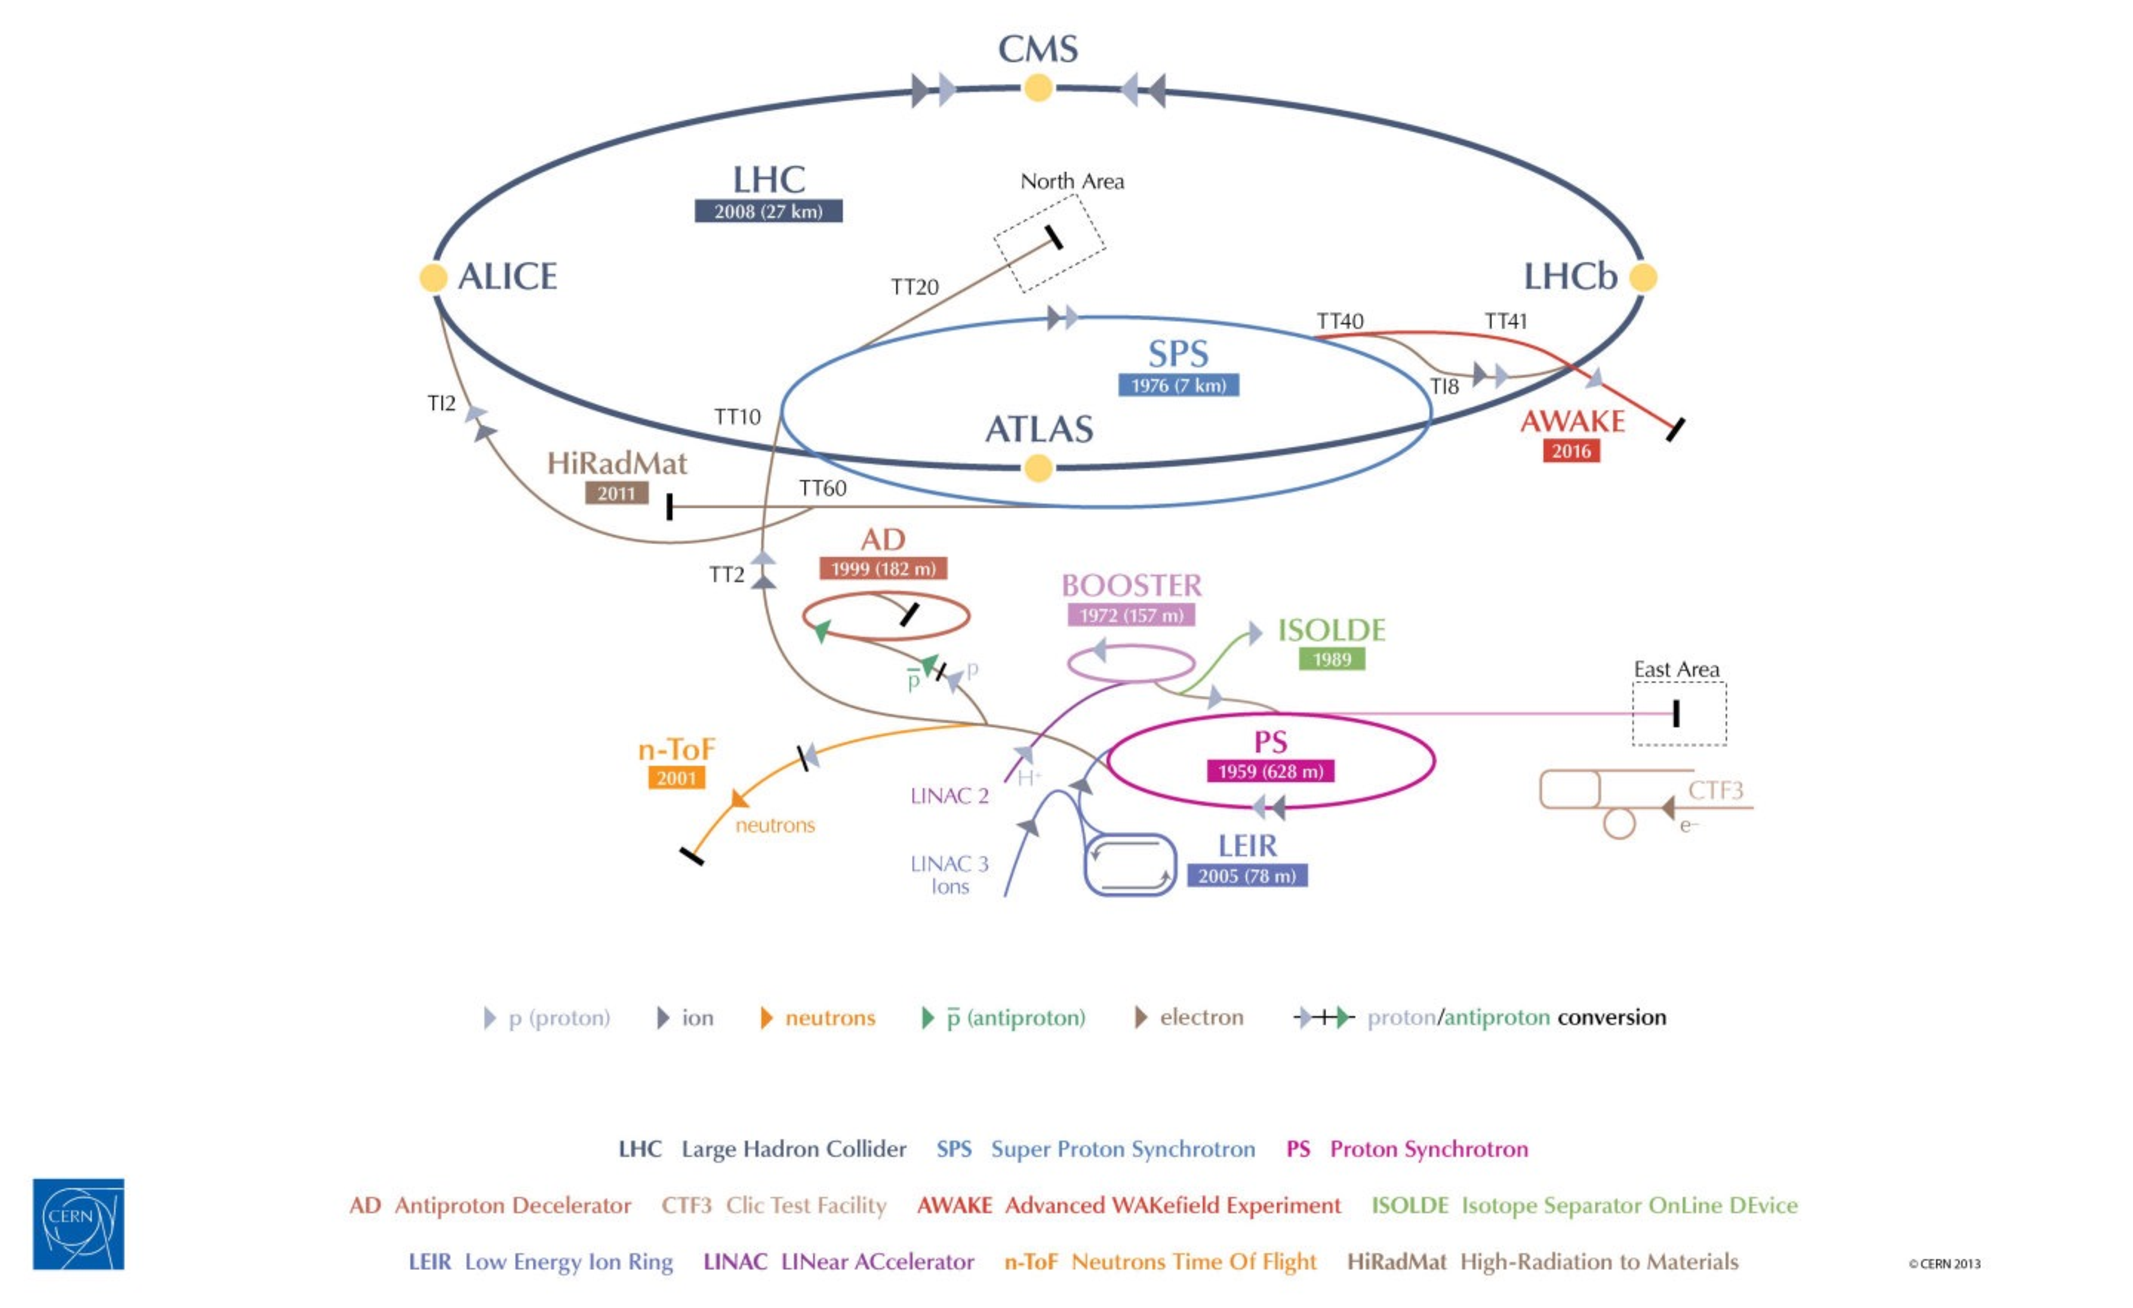
\includegraphics[width=\textwidth]{\chthree/LHC.pdf}
 \end{center}
 \caption{The CERN accelerator complex showing the chain of injection of protons into the LHC ring and the locations of the four main experiments ATLAS, CMS, LHCb and ALICE~\cite{Marcastel:1621583}.}
 \label{fig:LHC}
\end{figure}

LHC operation officially started at the beginning of September 2008 but it was interrupted after a short period, 
due to the breakdown of superconducting magnets. The collider has been reactivated in November 2009 with first pp collisions at $\sqrt{s} = 900\GeV$, officially starting a new era in the particle physics experiments. %Figure~\ref{fig:LHCschedule} shows the LHC timeline together with the phases of its operation. 
The operating center-of-mass energies in pp collisions have so far been 7\TeV in 2010-2011, 8\TeV in 2012 and 13\TeV in 2015-2016. The 7 and 8\TeV periods together make out the {\itshape LHC Run~1}, while the 13\TeV period is called the {\itshape LHC Run~2}. The work presented in this document is based on data sets collected with pp collisions at 8\TeV in 2012 and at 13\TeV in 2015.

During the whole Run~1, the LHC operated with a 50\unit{ns} bunch spacing.
The peak of instantaneous luminosity in 2011 has been $\approx 0.4\ten{34}\percms$ with a total delivered integrated luminosity of 6.1\fbinv~\cite{LumiPublicResults}.
In 2012 the beam energy increased to 4\TeV per beam with a peak luminosity of $\approx0.8\ten{34}\percms$ and 23.3\fbinv delivered integrated luminosity by the end of that year~\cite{LumiPublicResults}. The increment of the instantaneous luminosity leads to a no more negligible number of simultaneous interactions per bunch crossing, the so-called {\itshape pileup} (PU) events. It depends on the cross section of inelastic collisions (75\unit{mb} at $\sqrt{s} = 8\TeV$~\cite{Cartiglia:2013vsa}) and it is directly linked to the instantaneous luminosity. The average PU of the data collected in 2012 is equal to 21 (Fig.~\ref{fig:LHClumiAndPU}) while it has been around 15 in 2011~\cite{LumiPublicResults}.

A long shut-down period for the LHC (LS1) occurred during the whole 2013 and 2014, where upgrades and technical improvements have been performed in order to reach the designed instantaneous luminosity and center-of-mass energy. On March, 21st 2015 the first pp collisions at $\sqrt{s} = 13\TeV$ has been obtained, a new record-breaking energy. For the first three months the machine operated with 50\unit{ns} bunch spacing while, from August 2015, it has been reduced to the designed 25\unit{ns} and the number of bunches per beam has been increased. The first part of this Run~2 phase ended on November 2015 with a total delivered integrated luminosity of 4.2\fbinv and a peak luminosity of $\approx0.5\ten{34}\percms$ with an average pileup of 12~\cite{LumiPublicResults}.

The LHC Run~2 has been restarted in April 2016, after an end-of-the-year technical stop, reaching a peak luminosity of $\approx1.5\ten{34}\percms$. The machine has remained in operation at $\sqrt{s}$ = 13\TeV for the whole year with a total delivered integrated luminosity of 40\fbinv. Accordingly to the current LHC schedule, the Run~2 will proceed up to the end of 2018 with a total expected integrated luminosity of $\approx150\fbinv$. The data collected in 2016 are not considered in this work.

%\textcolor{red}{add some comments about HL-LHC}
%\begin{figure}[h]
% \begin{center}
%  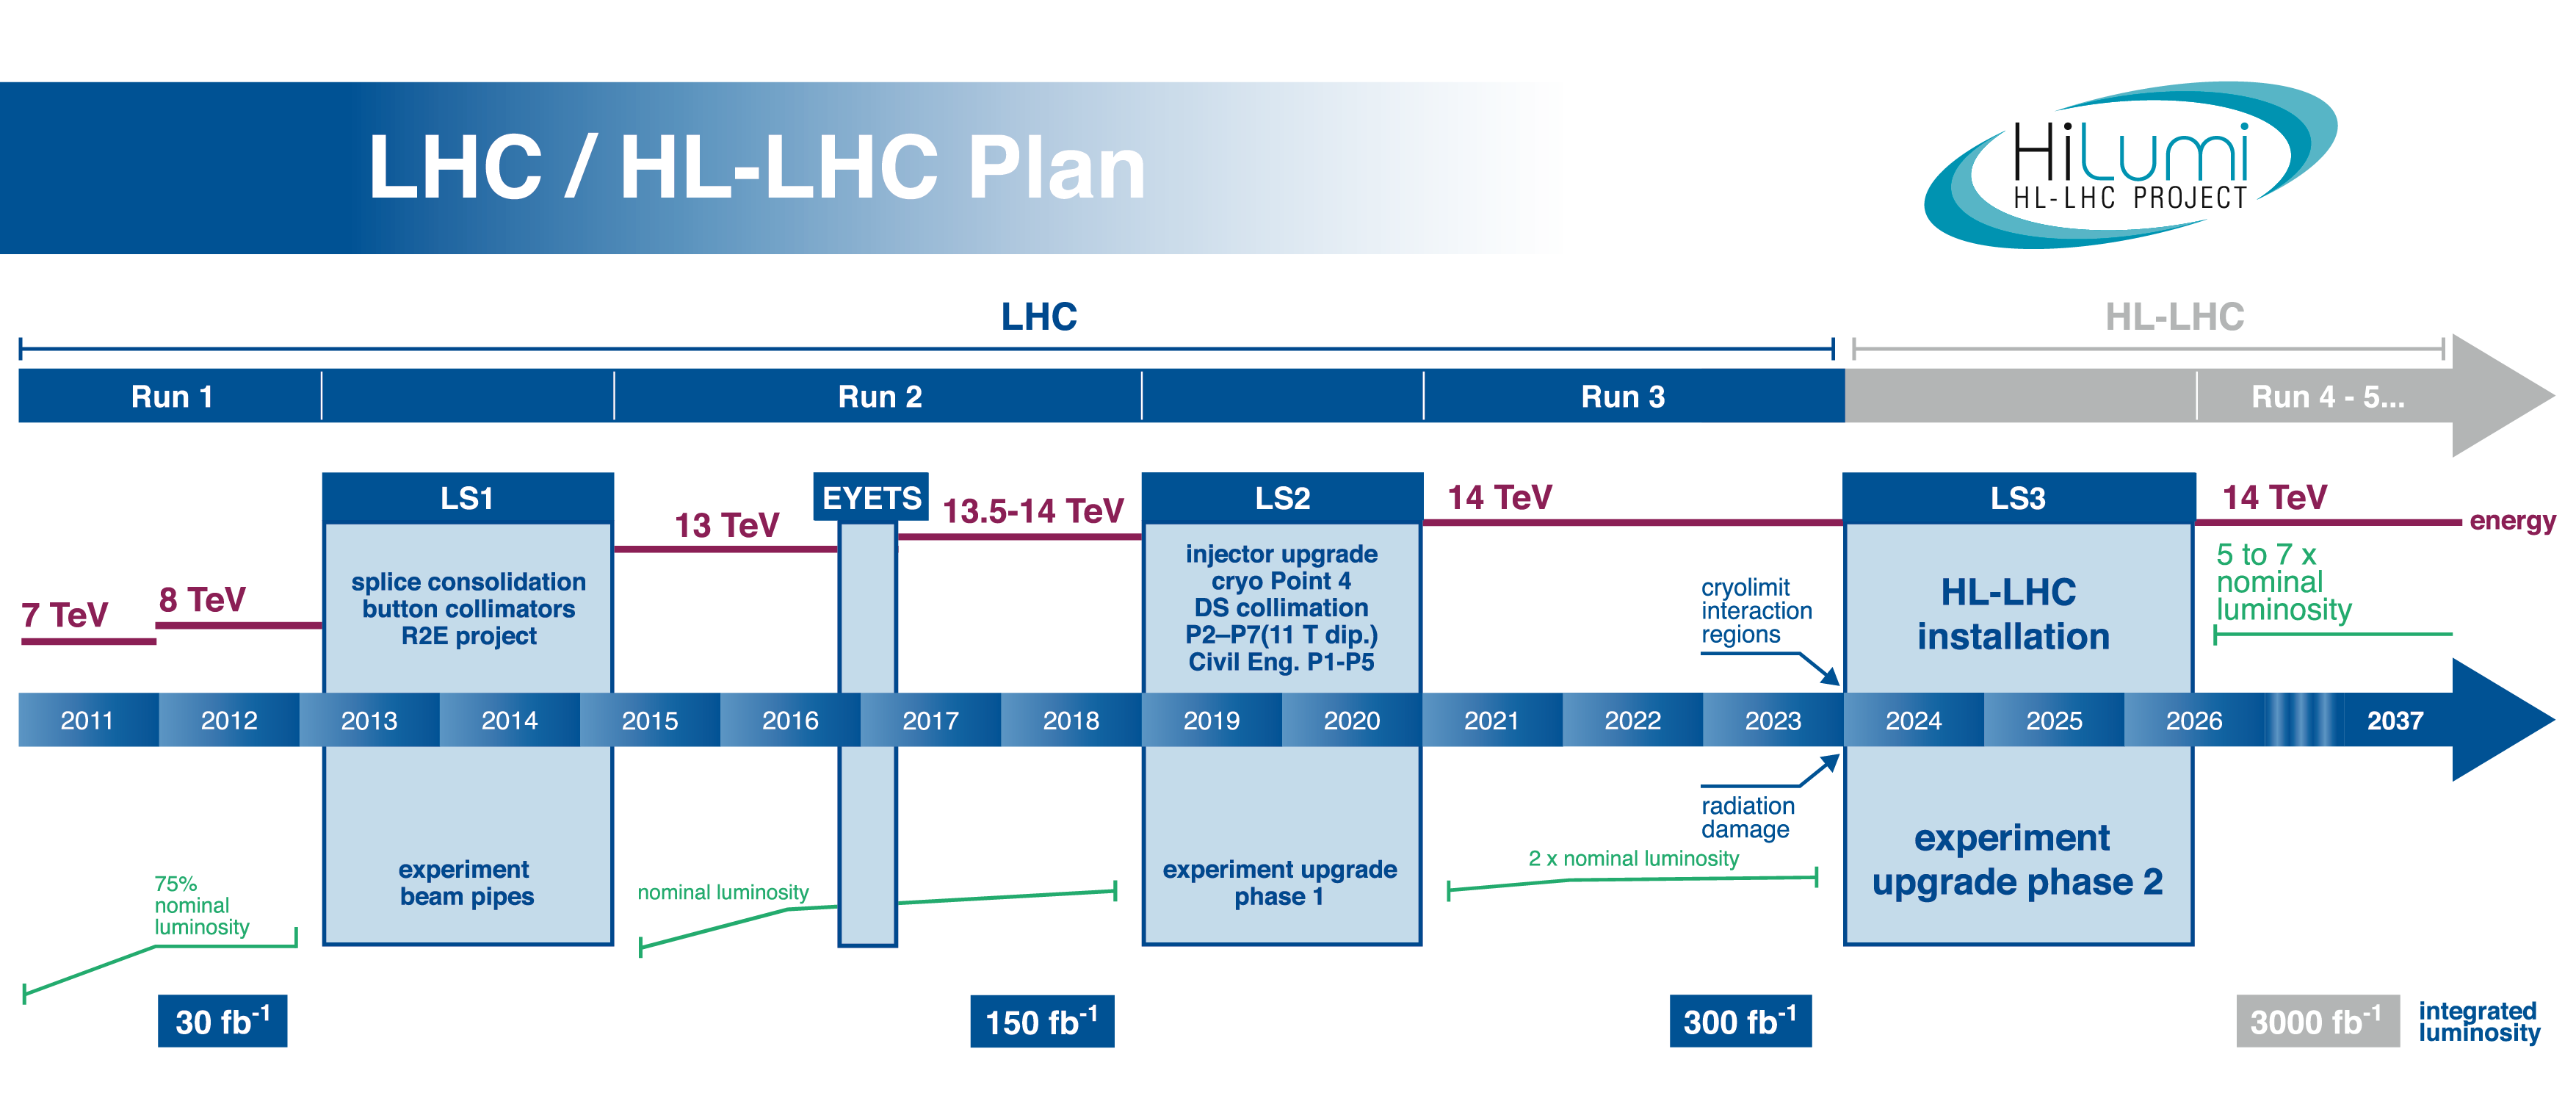
\includegraphics[width=\textwidth]{\chthree/HL-LHC-plan-2016-01.png}
% \end{center}
% \caption{LHC timeline.}
% \label{fig:LHCschedule}
%\end{figure}

\begin{figure}[!htb]
 \begin{center}
 \subfigure[]{\label{fig:LHClumiAndPU_a}\includegraphics[width=0.48\textwidth]{\chthree/pileup_pp_2012.png}}
 \subfigure[]{\label{fig:LHClumiAndPU_b}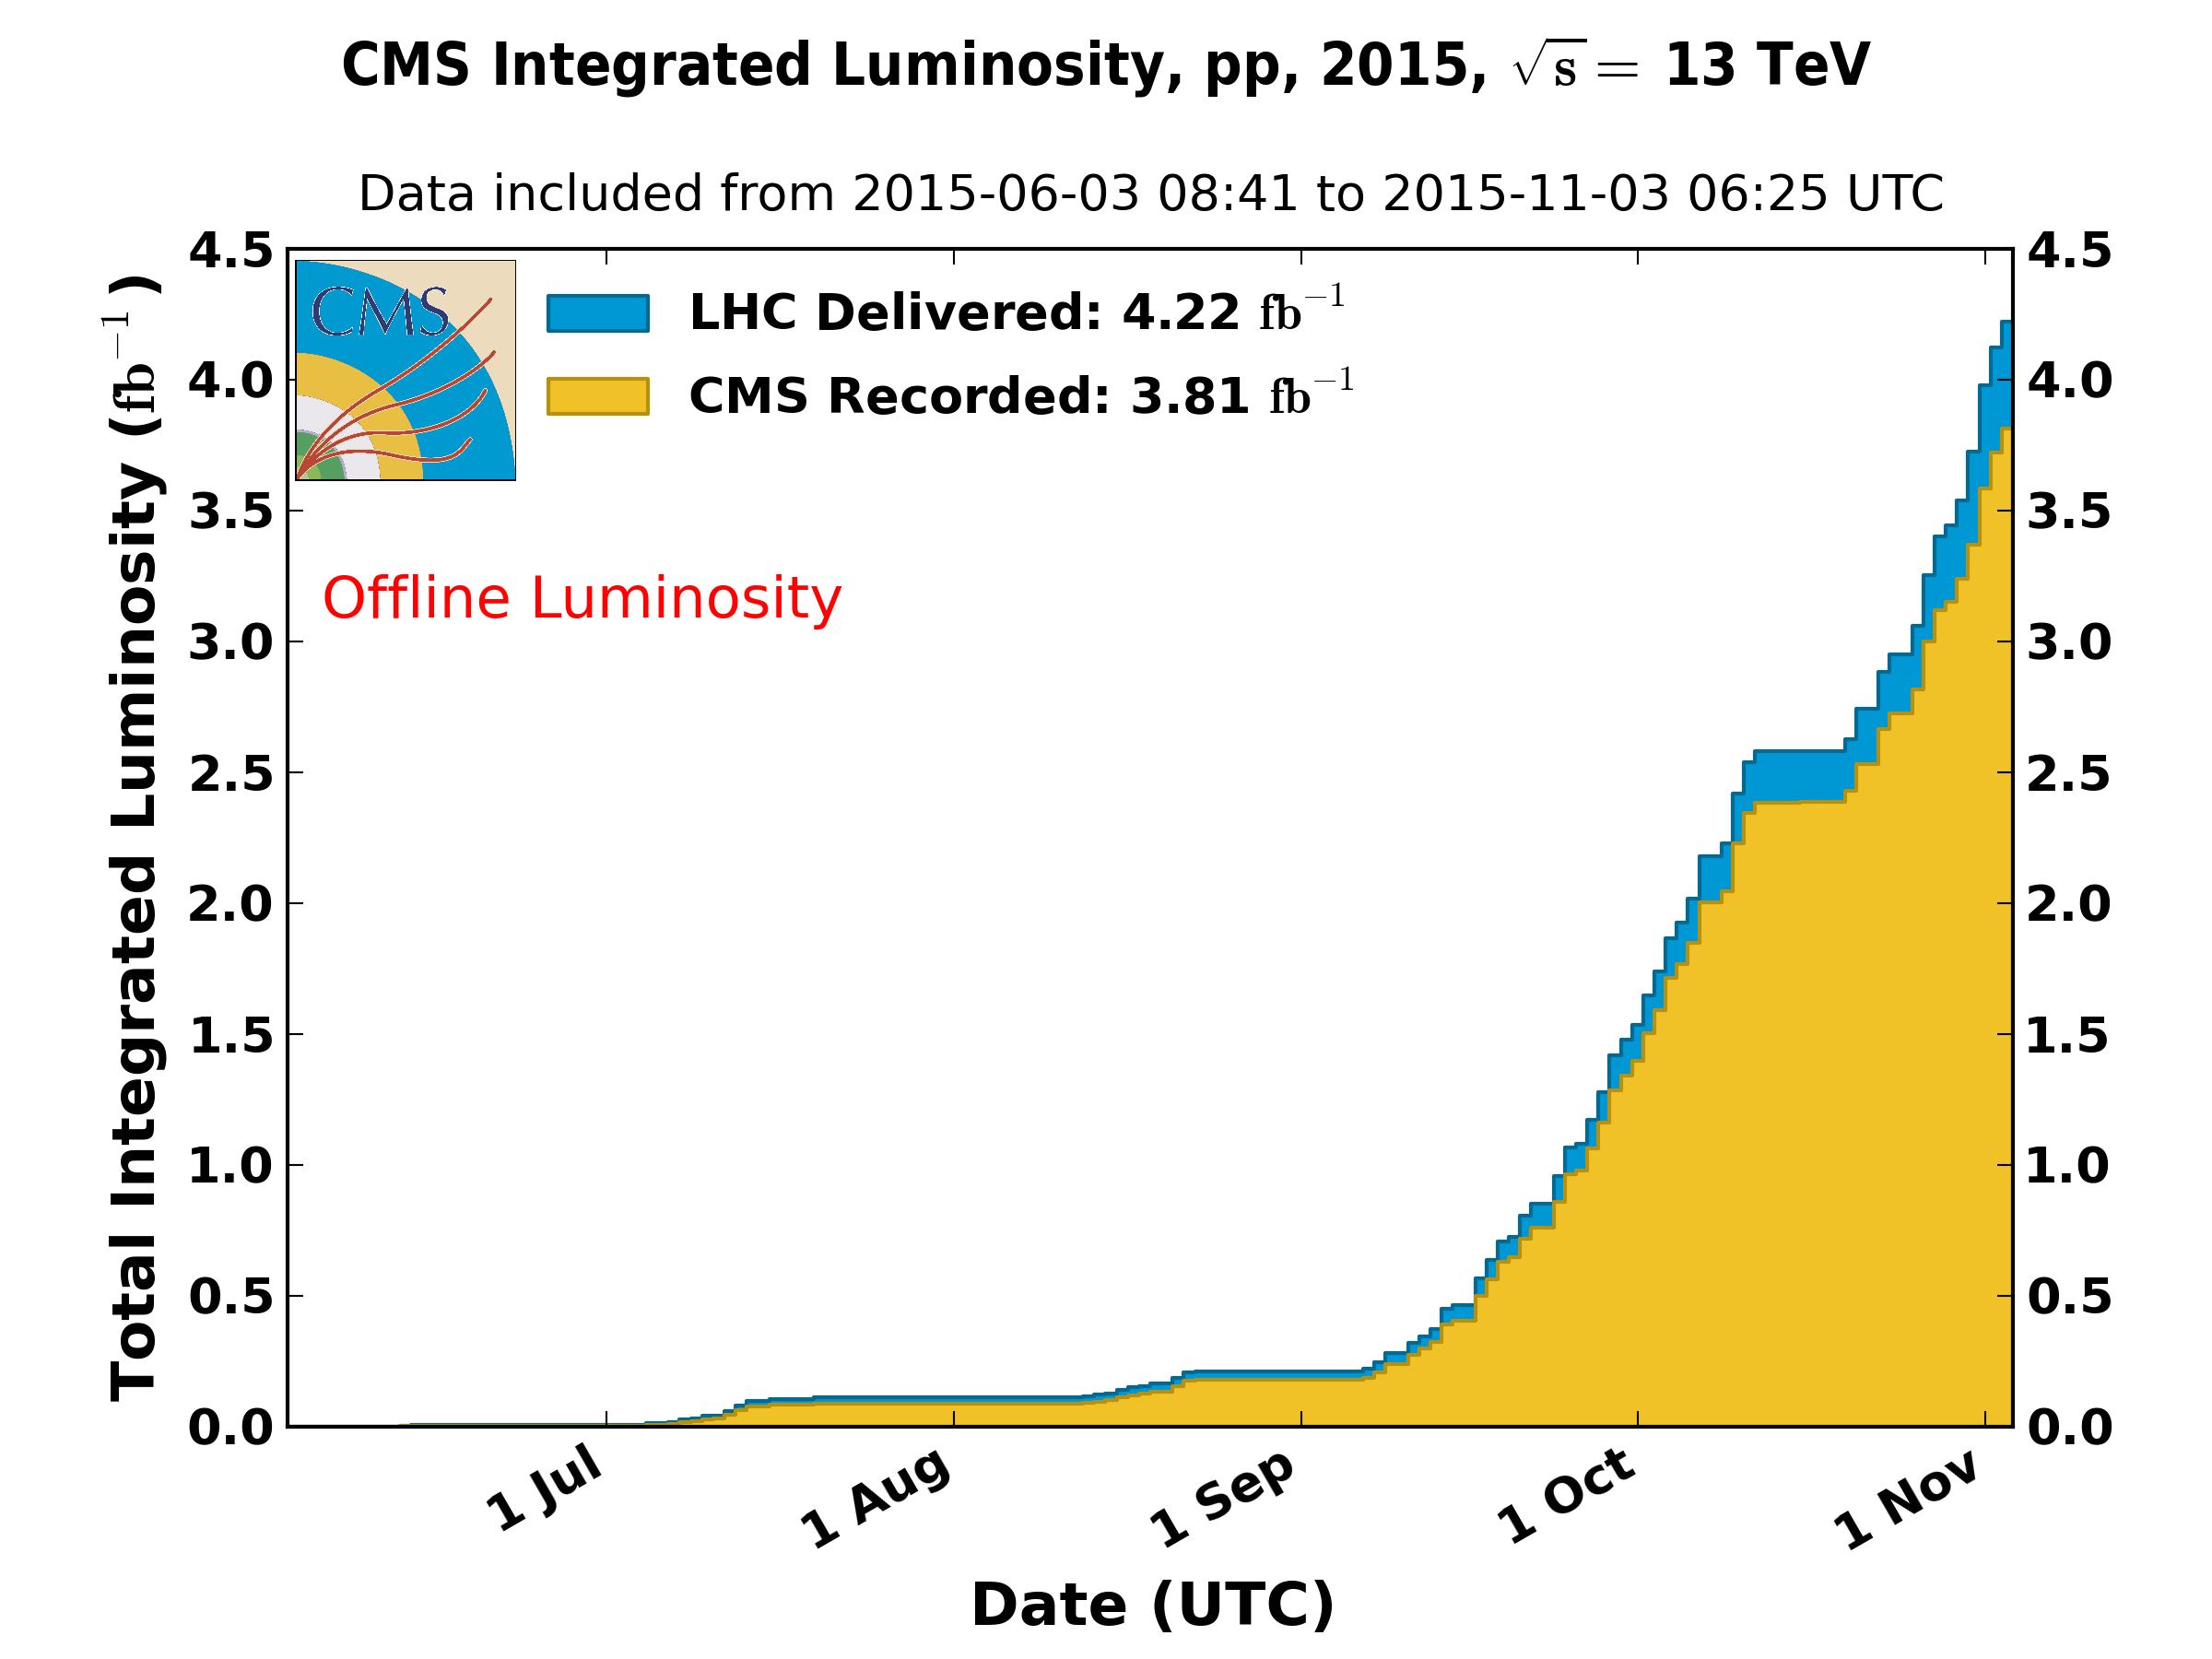
\includegraphics[width=0.48\textwidth]{\chthree/int_lumi_per_day_cumulative_pp_2015.png}}
 \end{center}
 \caption{(a) Number of simultaneous interactions per bunch crossing in data collected in 2012 by the CMS experiment at LHC. (b) Cumulative luminosity versus day delivered by LHC (blue) in 2015; the offline luminosity recorded by the CMS experiment is also reported (orange).~\cite{LumiPublicResults}}
 \label{fig:LHClumiAndPU}
\end{figure}

%\begin{figure}[h]
% \begin{center}
%  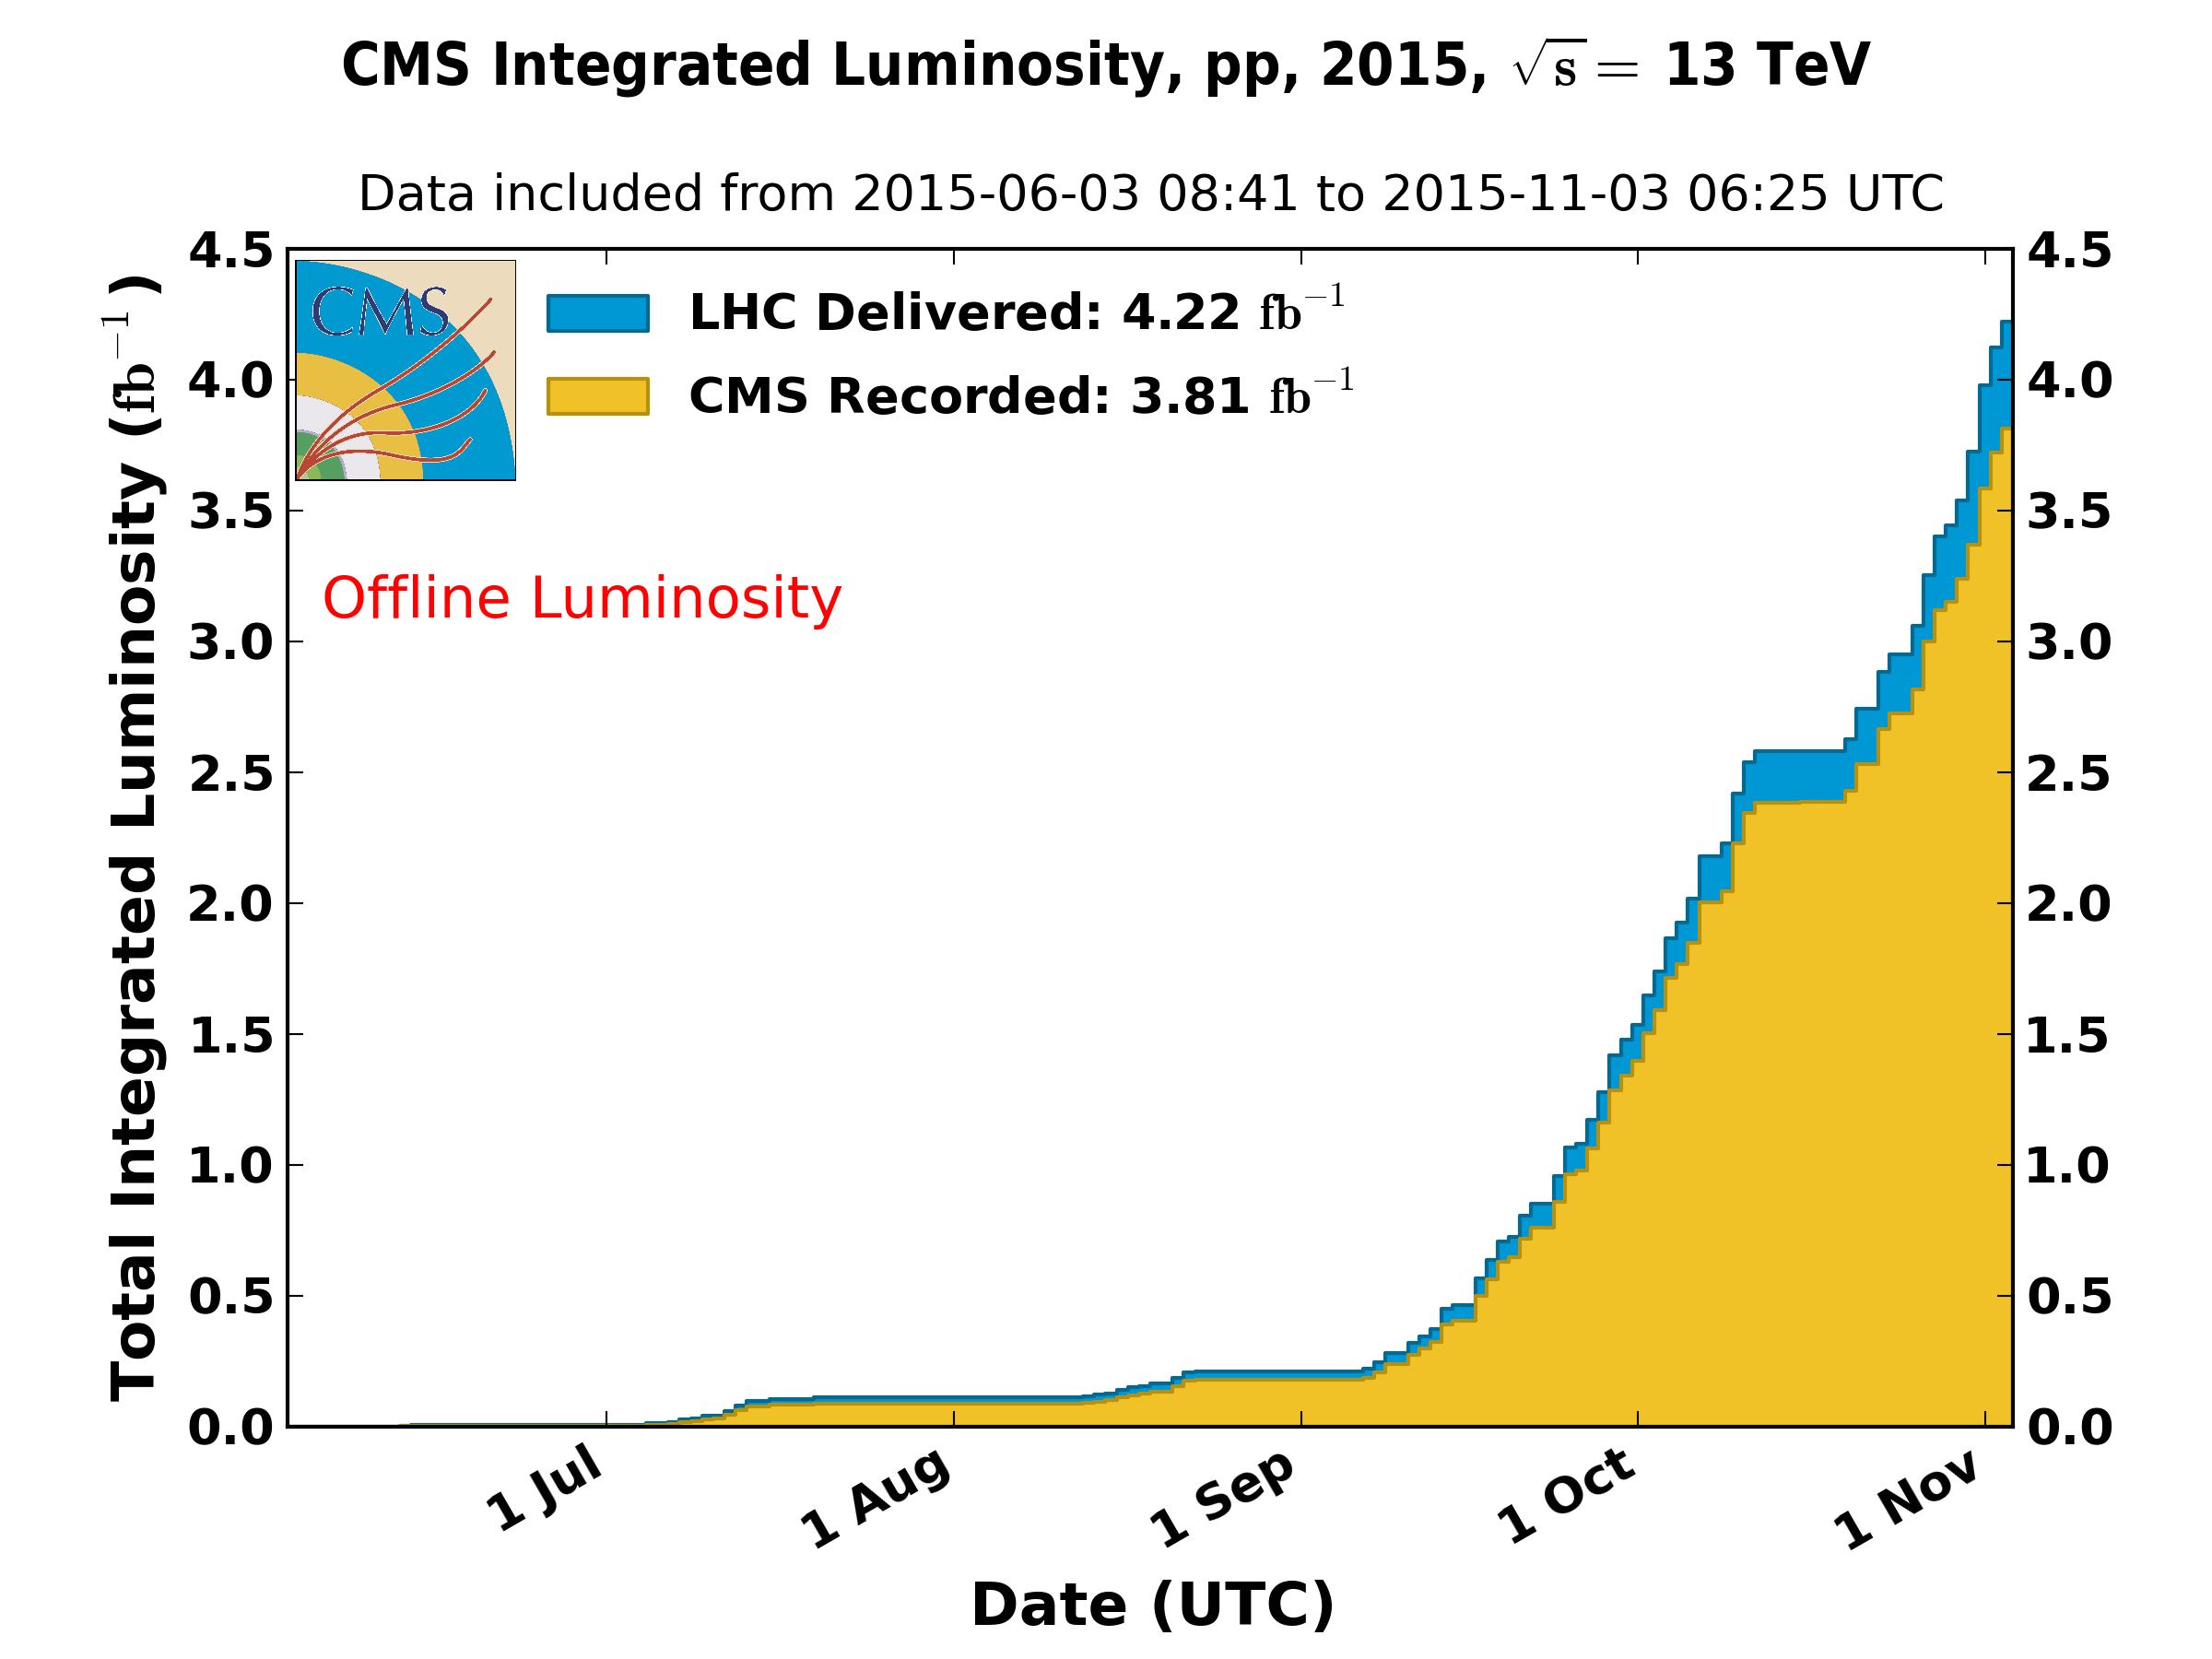
\includegraphics[width=0.45\textwidth]{\chthree/int_lumi_per_day_cumulative_pp_2015.png}
   %\includegraphics[height=11cm,width=0.5\textwidth]{chapters/Chapter3-CMSatLHC/Figurues/pileup_pp_2012.png}
% \end{center}
% \caption{Integrated lumi and PU for 2015.}
% \label{fig:LHCRun2}
%\end{figure}